\documentclass[10pt,twocolumn,letterpaper]{article}

\usepackage[top=1.8cm,bottom=1.8cm,left=1.8cm,right=1.8cm,columnsep=0.8cm]{geometry}
\usepackage{amsmath,amssymb,amsfonts}
\usepackage{newtxtext,newtxmath}
\usepackage{graphicx}
\usepackage{booktabs}
\usepackage{microtype}
\usepackage{xcolor}
\usepackage{tikz}
\usetikzlibrary{arrows.meta,positioning,shapes.geometric,calc}
\usepackage{enumitem}
\setlist{itemsep=0.6pt,topsep=1pt,parsep=0pt,partopsep=0pt,leftmargin=*}
\usepackage{titlesec}
\titleformat{\section}{\fontsize{11}{13}\selectfont\bfseries\color{darkcharcoal}}{}{0pt}{}
\titlespacing*{\section}{0pt}{4.5pt}{1.5pt}
\usepackage{cite}
\usepackage[colorlinks=true,linkcolor=teal!80!black,citecolor=teal!80!black,urlcolor=teal!80!black]{hyperref}

% Nature / Science editorial palette
\definecolor{natureblue}{RGB}{18, 72, 130}
\definecolor{natureteal}{RGB}{11, 145, 140}
\definecolor{crimsonaccent}{RGB}{186, 60, 45}
\definecolor{darkcharcoal}{RGB}{30, 35, 40}
\definecolor{palebg}{RGB}{246, 248, 250}
\definecolor{ambercolor}{RGB}{217, 130, 24}
\definecolor{cyancolor}{RGB}{14, 140, 180}

\newcommand{\headerbadge}[1]{%
  {\fontfamily{qcr}\selectfont\scriptsize\bfseries\color{natureteal}#1}%
}

\begin{document}

\twocolumn[{%
  \begin{minipage}{\textwidth}
  \vspace{-0.6cm}
  % \headerbadge{PERSPECTIVE / THEORETICAL FRAMEWORK}\par\vspace{0.06cm}
  {\fontsize{16.5}{20}\selectfont\bfseries\color{darkcharcoal} Vitrified Synapses in Superconducting Neuromorphic Circuits}\par\vspace{0.25cm}
  {\fontsize{11.5}{14}\selectfont\itshape\color{natureblue} Time-Resolved Cryo-ET Morphometry for Cryogenic Fluxon Circuits}\par\vspace{0.35cm}
  {\large\bfseries Erick Oduniyi}\par\vspace{0.08cm}
  {\small\itshape Massachusetts Institute of Technology, Cambridge, MA 02139, USA}\par
  {\small Correspondence: \texttt{erick000@media.mit.edu}}\par\vspace{0.3cm}
  \hrule height 0.8pt\vspace{0.25cm}
  {\small\textbf{Abstract}: Biological neural computation is intrinsically continuous, stochastic, and thermalized ($T \approx 310\,\text{K}$), evolving through ion channel gating, macromolecular rearrangements, and vesicle exocytosis. Conversely, superconducting electronics operate in the cryogenic domain ($T < 4.2\,\text{K}$), where single flux quanta (fluxons) in Josephson junction circuits produce non-linear conductance pulses with picosecond durations and sub-attojoule device switching energies ($\sim 0.2\,\text{aJ} = 2 \times 10^{-19}\,\text{J}$). Here, we propose a theoretical framework that connects time-resolved vitreous cryo-preservation with cryogenic neuromorphic circuit models. By arresting neuronal ensembles in vitreous ice via millisecond flash-and-freeze vitrification, cryo-electron tomography (cryo-ET) captures transient macromolecular configurations, including vesicle docking distances, fusion pore geometries, and postsynaptic receptor clustering. While a static ultrastructural snapshot cannot directly recover dynamical trajectories, we formulate a phenomenological parameter correspondence that maps reconstructed synaptic geometries into resistively shunted Josephson junction networks and magnetic Josephson synapses. We evaluate physical scaling boundaries, including refrigeration overhead and connectomic volume constraints, and discuss speculative public demonstrations designed for the MIT Museum.}\par\vspace{0.25cm}
  \hrule height 0.8pt\vspace{0.5cm}
  \end{minipage}
}]

\section*{1. Introduction: Synaptic Preservation}

A central problem in computational neuroscience and neuromorphic hardware is the physical representation of time. In biological nervous systems, cognitive processing unfolds along a continuous dynamical manifold governed by state-dependent, adaptive time constants~\cite{hasani2021liquid}:
\begin{equation}
\begin{aligned}
  \frac{d\mathbf{x}(t)}{dt} = &-\left[\frac{1}{\tau_0} + f(\mathbf{x}(t), \mathbf{I}(t), \theta)\right]\mathbf{x}(t) \\
  &+ f(\mathbf{x}(t), \mathbf{I}(t), \theta)\mathbf{A} + \mathbf{W}_{\text{in}}\mathbf{I}(t),
\end{aligned}
\label{eq:neural_ode}
\end{equation}
where $\mathbf{x}(t) \in \mathbb{R}^D$ denotes the hidden state vector, $\tau_0$ is the baseline leakage timescale, $\mathbf{A}$ represents a resting state vector, and $f(\cdot)$ is a bounded non-linear function modulating the effective synaptic conductance from inputs $\mathbf{I}(t)$ and recurrent interactions.

To resolve transient biophysical conformations along this manifold at nanometer scale, physical motion must be arrested without introducing chemical cross-linking distortions. Conventional aldehyde fixation causes protein denaturation and requires seconds to minutes, smearing fast physiological events.

By contrast, \textbf{cryo-vitrification} cools aqueous specimens at rates exceeding $10^5\,\text{K/s}$, preventing water molecules from organizing into a crystalline lattice. Instead, water solidifies into amorphous \textbf{vitreous ice}~\cite{watanabe2013flash}. Plunge freezing into liquid ethane ($T \approx 90\,\text{K}$) vitrifies thin specimens ($\lesssim 10\,\mu\text{m}$, such as synaptosomes or monolayer cultures), whereas thicker intact neural tissue requires high-pressure freezing (HPF, $\sim 2000\,\text{bar}$) to vitrify up to $200\,\mu\text{m}$. When synchronized with optogenetic stimulation (\textit{flash-and-freeze}), vitrification preserves transient intermediate configurations at defined latencies following an action potential~\cite{watanabe2018synaptic,imig2014ultrastructural}.

Concurrently, neuromorphic engineering seeks physical substrates capable of evaluating continuous non-linear differential equations with minimal dissipation. Superconducting electronics operate below the critical temperature of niobium ($T_c = 9.2\,\text{K}$, typically in liquid helium at $4.2\,\text{K}$ or sub-Kelvin). At these temperatures, quantized magnetic fluxons propagate through Josephson transmission lines at picosecond timescales with junction switching energies on the order of $10^{-19}\,\text{J}$~\cite{crotty2010josephson,schneider2018ultralow}.

Vitrified biological tissue and superconducting circuits share a low-temperature operational regime. However, this temperature overlap is not an active computational coupling: vitrified tissue is metabolically inert. Rather, the cryogenic environment provides an engineering common ground. Ultrastructural parameters reconstructed from cryo-ET can directly parameterize cryogenic superconducting circuits without thermal translation artifacts. 

\begin{figure*}[t]
\centering
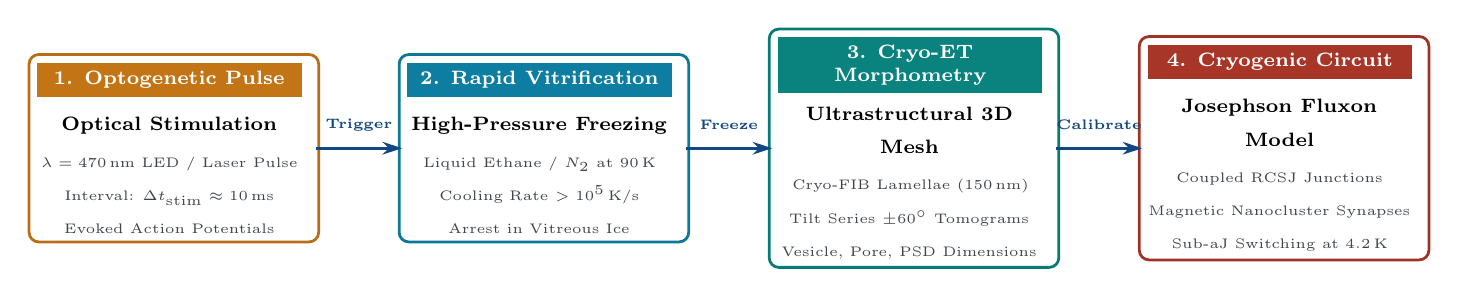
\begin{tikzpicture}[
    card/.style={draw=darkcharcoal!35, fill=white, rounded corners=3.5pt, line width=1pt, minimum width=3.5cm, minimum height=1.95cm, inner sep=3pt, align=center},
    arrow/.style={-{Stealth[length=2.5mm, width=1.6mm]}, line width=1.1pt, color=natureblue}
]

% 4 Cards: Centers at 1.75, 6.45, 11.15, 15.85 (Width=3.5cm, Gaps=1.2cm)
% Card 1: Optogenetic Stimulation
\node[card, draw=ambercolor!85!black] (c1) at (1.75, 0) {
  \begin{minipage}{3.35cm}
  \centering
  \colorbox{ambercolor!90!black}{\parbox{3.15cm}{\centering\scriptsize\bfseries\color{white}1. Optogenetic Pulse}}\par\vspace{0.14cm}
  {\scriptsize\textbf{Optical Stimulation}}\par\vspace{0.04cm}
  {\tiny\color{darkcharcoal!85} $\lambda = 470$\,nm LED / Laser Pulse}\par
  {\tiny\color{darkcharcoal!85} Interval: $\Delta t_{\text{stim}} \approx 10$\,ms}\par
  {\tiny\color{darkcharcoal!85} Evoked Action Potentials}
  \end{minipage}
};

% Card 2: Rapid Vitrification
\node[card, draw=cyancolor!85!black] (c2) at (6.45, 0) {
  \begin{minipage}{3.35cm}
  \centering
  \colorbox{cyancolor!90!black}{\parbox{3.15cm}{\centering\scriptsize\bfseries\color{white}2. Rapid Vitrification}}\par\vspace{0.14cm}
  {\scriptsize\textbf{High-Pressure Freezing}}\par\vspace{0.04cm}
  {\tiny\color{darkcharcoal!85} Liquid Ethane / $N_2$ at $90$\,K}\par
  {\tiny\color{darkcharcoal!85} Cooling Rate $> 10^5$\,K/s}\par
  {\tiny\color{darkcharcoal!85} Arrest in Vitreous Ice}
  \end{minipage}
};

% Card 3: Cryo-ET Morphometry
\node[card, draw=natureteal!85!black] (c3) at (11.15, 0) {
  \begin{minipage}{3.35cm}
  \centering
  \colorbox{natureteal!90!black}{\parbox{3.15cm}{\centering\scriptsize\bfseries\color{white}3. Cryo-ET Morphometry}}\par\vspace{0.14cm}
  {\scriptsize\textbf{Ultrastructural 3D Mesh}}\par\vspace{0.04cm}
  {\tiny\color{darkcharcoal!85} Cryo-FIB Lamellae ($150$\,nm)}\par
  {\tiny\color{darkcharcoal!85} Tilt Series $\pm 60^\circ$ Tomograms}\par
  {\tiny\color{darkcharcoal!85} Vesicle, Pore, PSD Dimensions}
  \end{minipage}
};

% Card 4: Superconducting Emulation
\node[card, draw=crimsonaccent!85!black] (c4) at (15.85, 0) {
  \begin{minipage}{3.35cm}
  \centering
  \colorbox{crimsonaccent!90!black}{\parbox{3.15cm}{\centering\scriptsize\bfseries\color{white}4. Cryogenic Circuit}}\par\vspace{0.14cm}
  {\scriptsize\textbf{Josephson Fluxon Model}}\par\vspace{0.04cm}
  {\tiny\color{darkcharcoal!85} Coupled RCSJ Junctions}\par
  {\tiny\color{darkcharcoal!85} Magnetic Nanocluster Synapses}\par
  {\tiny\color{darkcharcoal!85} Sub-aJ Switching at $4.2$\,K}
  \end{minipage}
};

% Connections: Gaps are 1.2cm long (3.5 to 4.7, 8.2 to 9.4, 12.9 to 14.1)
\draw[arrow] (3.55, 0) -- (4.65, 0);
\node[font=\tiny\bfseries\color{natureblue}] at (4.1, 0.3) {Trigger};

\draw[arrow] (8.25, 0) -- (9.35, 0);
\node[font=\tiny\bfseries\color{natureblue}] at (8.8, 0.3) {Freeze};

\draw[arrow] (12.95, 0) -- (14.05, 0);
\node[font=\tiny\bfseries\color{natureblue}] at (13.5, 0.3) {Calibrate};

\end{tikzpicture}
\vspace{0.08cm}
\caption{\textbf{Vitrified-to-superconducting experimental pipeline.} Cultured neurons or brain tissue are optogenetically stimulated and vitrified at millisecond intervals ($\Delta t_{\text{freeze}} \in [5, 100]$\,ms) into vitreous ice. Cryo-focused ion beam (cryo-FIB) milling and cryo-electron tomography (cryo-ET) resolve nanometer-scale synaptic architectures. Reconstructed morphometrics calibrate analog parameters in superconducting Josephson junction models and magnetic fluxon synapses.}
\label{fig:pipeline}
\vspace{-0.3cm}
\end{figure*}

\section*{2. Time-Resolved Cryo-ET Morphometry}

In high-pressure freezing (HPF) and plunge-freezing workflows, cultured hippocampal or cortical networks expressing light-gated channelrhodopsin-2 (ChR2) are mounted on electron microscopy grids. Following an optical pulse ($\Delta t_{\text{stim}} \approx 10\,\text{ms}$), samples are frozen at controlled latencies $\Delta t_{\text{freeze}} \in [5, 100]\,\text{ms}$. Thin lamellae ($150 - 200\,\text{nm}$) prepared by cryogenic focused ion beam (cryo-FIB) milling are imaged via cryo-electron tomography (cryo-ET) across tilt series of $\pm 60^\circ$~\cite{imig2014ultrastructural}.

Three-dimensional tomographic reconstructions with subtomogram averaging resolve quantitative structural markers of instantaneous synaptic state:

\begin{enumerate}
  \item \textbf{Vesicle Proximity and SNARE Assembly:} The spatial distance $d_v$ of synaptic vesicles from the active zone plasma membrane, identifying docked vesicles ($d_v < 5\,\text{nm}$) within the readily releasable pool and trans-SNARE complexes (syntaxin-1, SNAP-25, synaptobrevin-2) paired with synaptotagmin-1 $\text{Ca}^{2+}$ sensors.
  \item \textbf{Fusion Pore Apertures:} The neck radius $r_{\text{pore}} \in [1, 5]\,\text{nm}$ of arrested fusion intermediates, capturing transient pore formation before full-collapse exocytosis.
  \item \textbf{Active Zone Protein Scaffolding:} Macromolecular cluster positions of Bassoon, Piccolo, and RIM that organize voltage-gated calcium channels (VGCCs) relative to release sites.
  \item \textbf{Postsynaptic Density (PSD) Area and Clustering:} The surface area $A_{\text{PSD}}$ and packing density of ionotropic AMPA and NMDA receptor complexes anchored by PSD-95 scaffolding across the $\sim 20\,\text{nm}$ synaptic cleft.
\end{enumerate}

These measurements capture instantaneous structural snapshots. However, cryo-ET lamellae sample a local volume ($< 0.2\,\mu\text{m}$ thick), and milling destroys the adjacent tissue. Consequently, cryo-ET resolves nanoscale synaptic components, but tracing long-range connectivity requires complementary volume electron microscopy (such as serial-section EM or FIB-SEM).

\section*{3. Superconducting Josephson Dynamics}

Superconducting neuromorphic circuits exploit macroscopic quantum phase coherence in Josephson junctions. A junction comprises two superconducting electrodes (e.g., Nb) separated by a thin barrier (e.g., $\text{AlO}_x$). The quantum phase difference $\phi(t) = \theta_1 - \theta_2$ dictates the supercurrent through the dc Josephson relation $I_s = I_c \sin\phi$. 

Under the standard \textbf{Resistively and Capacitively Shunted Josephson (RCSJ)} model~\cite{stewart1968current,mccumber1968effect}:
\begin{equation}
  \frac{\hbar C}{2e} \frac{d^2\phi}{dt^2} + \frac{\hbar}{2e R} \frac{d\phi}{dt} + I_c \sin\phi = I_{\text{bias}}(t),
  \label{eq:rcsj}
\end{equation}
where $C$ is junction capacitance, $R$ is shunt resistance, $I_c$ is critical current, and $e$ is elementary charge.

\begin{table*}[t]
\centering
\small
\caption{\textbf{Physical and Computational Synaptic Metrics across Biological and Superconducting Domains}}
\vspace{0.06cm}
\begin{tabular}{@{}lll@{}}
\toprule
\textbf{Metric} & \textbf{Biological Synapse} & \textbf{Superconducting Fluxon Synapse} \\
\midrule
Operating Temperature ($T$) & $310\,\text{K}$ (37$^\circ$C) & $4.2\,\text{K}$ (Liquid Helium) / sub-1K \\
Signal Carrier & $\text{Ca}^{2+}, \text{Na}^+, \text{K}^+$ ions & Cooper pairs / Magnetic fluxons ($\Phi_0 = h/2e$) \\
Pulse Duration & $1 - 5\,\text{ms}$ (action potential) & $1 - 5\,\text{ps}$ (single flux quantum) \\
Device Switching Energy & $\sim 1 - 10\,\text{fJ}$ ($10^{-14}\,\text{J}$, ATP turnover) & $\sim 0.2\,\text{aJ}$ ($2 \times 10^{-19}\,\text{J}$, on-chip junction energy) \\
Refrigeration Overhead ($4.2\,\text{K}$) & None (ambient physiological) & $\sim 500 - 1000\,\text{W/W}$ ($\sim 0.1 - 0.2\,\text{fJ}$ wall-plug equivalent) \\
State Representation & Vesicle docking proximity / PSD area & Remanent magnetic cluster state / trapped fluxoid \\
Physical Substrate & Vitreous ice / cellular membranes & Superconducting $\text{Nb/Al-AlO}_x\text{/Nb}$ and $\text{Nb/Si:Mn/Nb}$ thin films \\
\bottomrule
\end{tabular}
\label{tab:metrics}
\end{table*}

Equation~\ref{eq:rcsj} is formally analogous to a driven, damped physical pendulum in a tilted periodic potential. While a single junction provides a second-order phase equation, emulating the full four-dimensional dynamics of the biological Hodgkin-Huxley model (with separate activation, inactivation, and refractory mechanisms) requires circuits of two or more inductively or resistively coupled junctions~\cite{crotty2010josephson}:
\begin{itemize}
  \item The junction phase trajectory $\phi(t)$ relates to terminal voltage through the ac Josephson relation $V(t) = \frac{\hbar}{2e} \frac{d\phi}{dt}$.
  \item When input bias current triggers a $2\pi$-phase slip, the junction generates a quantized Single Flux Quantum (SFQ) voltage pulse:
  \begin{equation}
    \int V(t)\,dt = \Phi_0 = \frac{h}{2e} \approx 2.068 \times 10^{-15}\,\text{Wb}.
  \end{equation}
  \item An SFQ pulse has a picosecond duration ($\sim 1 - 2\,\text{ps}$) and peak amplitude $\sim 1\,\text{mV}$.
  \item The on-chip energy dissipated during a single junction switching event is bounded by:
  \begin{equation}
    E_{\text{SFQ}} \approx I_c \Phi_0 \approx (100\,\mu\text{A})(2.07 \times 10^{-15}\,\text{Wb}) \approx 0.2\,\text{aJ},
  \end{equation}
  which is roughly $2 \times 10^{-19}\,\text{J}$ ($0.2\,\text{aJ}$), approximately four orders of magnitude below the metabolic cost of a biological synaptic release event ($\sim 10\,\text{fJ}$~\cite{attwell2001energy}) and three to four orders below modern CMOS logic gates ($0.1 - 1\,\text{fJ}$).
  \item \textbf{Refrigeration Cost:} Any cryogenic electronic technology must account for cooling overhead. At $4.2\,\text{K}$, Carnot limits and practical cryocooler efficiencies impose an overhead factor of $\beta_{\text{cool}} \approx 500 - 1000\,\text{W}$ of electrical input per watt of cryogenic heat removal~\cite{holmes2013energy}. Including this factor, an on-chip $0.2\,\text{aJ}$ event consumes $\sim 0.1 - 0.2\,\text{fJ}$ of wall-plug energy, remaining competitive with room-temperature CMOS while operating at multi-gigahertz clock frequencies.
\end{itemize}

\section*{4. Ultrastructure-to-Circuit Mapping}

Rather than claiming a formal category-theoretic isomorphism, we formulate a phenomenological parameter correspondence mapping measured 3D ultrastructural features to circuit components:

\begin{enumerate}
  \item \textbf{Conductance to Critical Current ($g_{\text{syn}} \mapsto I_c$):} The postsynaptic density area $A_{\text{PSD}}$ and AMPA/NMDA receptor density calibrate the effective critical current $I_c \propto A_{\text{PSD}}$ of an input coupling junction, establishing the threshold current required to emit an SFQ pulse.
  \item \textbf{Vesicle Proximity to Damping Parameter ($d_v \mapsto \beta_c$):} The spatial proximity $d_v$ of docked vesicles regulates release probability in biology. In the circuit model, this maps to the Stewart-McCumber damping parameter $\beta_c = \frac{2e I_c R^2 C}{\hbar}$, which determines whether the junction exhibits hysteretic (underdamped, bistable) or non-hysteretic (overdamped) switching.
  \item \textbf{Synaptic Weighting via Magnetic Josephson Junctions (MJJs):} Non-volatile analog synaptic weights are implemented using Magnetic Josephson Junctions containing magnetic nanoclusters (e.g., Mn-doped silicon barriers, $\text{Nb/Si}_{1-x}\text{Mn}_x\text{/Nb}$)~\cite{schneider2018ultralow}. Modulating the remanent magnetic order of the barrier tunes $I_c$ continuously across a wide dynamic range, providing an energy-efficient non-volatile memory cell that operates at $4.2\,\text{K}$.
  \item \textbf{Timescale Scaling ($\alpha \sim 10^7$):} Individual SFQ pulses are roughly $10^9\times$ shorter than biological action potentials ($1\,\text{ps}$ vs $1\,\text{ms}$). At the network integration level, superconducting circuits clock between $20 - 50\,\text{GHz}$, whereas biological firing frequencies are $10 - 100\,\text{Hz}$. Thus, dynamical integration of an analog neural ODE state that requires seconds in biology can be evaluated in sub-microsecond timescales on cryogenic hardware.
  \item \textbf{Inversion Limits:} A single cryo-ET snapshot records an arrested structural configuration $\mathbf{x}(t^*)$, but cannot uniquely identify time-varying parameters such as recurrent connectivity matrices $\mathbf{W}_{\text{rec}}$ or dynamic leakage terms $\tau(\cdot)$ in Equation~\ref{eq:neural_ode}. The structural data provide boundary conditions and parameter priors rather than a direct reconstruction of ongoing cognitive activity.
\end{enumerate}

\section*{5. Cryogenic Quantum Characterization}

Beyond parameter mapping, we consider the direct characterization of vitrified neural tissue at cryogenic temperatures using quantum sensing probes:

\begin{itemize}
  \item \textbf{NanoSQUID Magnetometry:} Sub-micron Superconducting Quantum Interference Devices (nanoSQUIDs) fabricated from nanoscale constriction junctions achieve spin sensitivities on the order of $\sim 1\,\mu_{\text{B}}/\sqrt{\text{Hz}}$~\cite{anahory2020squid}. Positioned above a cryo-FIB vitrified neural lamella maintained below $10\,\text{K}$, nanoSQUIDs can map local stray magnetic fields arising from metalloprotein distributions (such as ferritin iron cores) without warming or chemically modifying the sample.
  \item \textbf{Cryogenic Scanning Microwave Microscopy (SMM):} A superconducting transmission line resonator coupled to a cryogenic probe tip enables localized dielectric spectroscopy at tens-of-nanometers spatial resolution, measuring complex permittivity $\epsilon_r$ across vitrified cell membranes and protein assemblies.
\end{itemize}

\section*{6. MIT Museum Gallery Installations}

For public science communication at the MIT Museum, this theoretical intersection between vitrified biology and superconducting electronics provides the foundation for two speculative gallery installations:

\begin{enumerate}
  \item \textbf{The Frozen Synapse Visualizer:} An interactive volumetric display rendering real cryo-ET tomograms of vitrified synapses. Visitors navigate 3D reconstructions of vitreous ice, examining docked vesicles, fusion pores, and postsynaptic scaffolding proteins.
  \item \textbf{The Cryo-Neuromorphic Interactive Console:} A speculative physical interface featuring aluminum rotary dials, patch cables, and thermal indicators that visualizes phase transitions across temperature:
  \begin{itemize}
    \item \textbf{Physiological ($310\,\text{K}$):} Stochastic, warm biological rhythms modeled by continuous Neural ODEs.
    \item \textbf{Vitrified ($90\,\text{K}$):} Structural motion freezes into static vitreous ice; dynamical updates halt.
    \item \textbf{Superconducting ($4.2\,\text{K}$):} Ballistic fluxon emission generates rapid pulse trains, sonifying ultra-fast cryogenic circuit dynamics.
  \end{itemize}
\end{enumerate}

\section*{7. Conclusion}

Vitrified structural biology and superconducting neuromorphic engineering operate on complementary ends of the dynamical spectrum. While time-resolved cryo-ET arrests biological synaptic configurations in vitreous ice to provide quantitative macromolecular priors, superconducting Josephson circuits offer an ultra-low-energy, high-bandwidth physical substrate for executing continuous non-linear neural dynamics. Recognizing both the potential and the physical boundaries of this correspondence clarifies the path toward hybrid biophysical modeling and cryogenic quantum computing.

\footnotesize
\begin{thebibliography}{99}
\setlength{\itemsep}{-0.5pt}
\setlength{\parskip}{0pt}
\bibitem{hasani2021liquid} R. Hasani, M. Lechner, A. Amini, D. Rus, R. Grosu, ``Liquid Time-constant Networks,'' \textit{Nature Machine Intelligence}, vol. 3, pp. 148--160, 2021.
\bibitem{watanabe2013flash} S. Watanabe, B. R. Rost, M. Camacho-P{\'e}rez, C. Davis, B. S{\"o}hl-Kielczynski, C. M. Felies, C. Rosenmund, E. M. Jorgensen, ``Ultrafast endocytosis at mouse hippocampal synapses,'' \textit{Nature}, vol. 504, pp. 242--247, 2013.
\bibitem{watanabe2018synaptic} S. Watanabe, N. Mamer, S. Raychaudhuri, N. Luvsanjav, J. Eisen, D. Trimbuch, B. S{\"o}hl-Kielczynski, M. W. Fenske, I. Milosevic, C. Rosenmund, E. M. Jorgensen, ``Synaptic vesicle exocytosis and endocytosis in human pluripotent stem cell-derived neurons,'' \textit{Elife}, vol. 7, e39718, 2018.
\bibitem{imig2014ultrastructural} C. Imig, S. W. Min, S. Krinner, M. Arancillo, C. Rosenmund, T. C. S{\"u}dhof, J. Rhee, N. Brose, B. H. Cooper, ``The morphological and molecular nature of synaptic vesicle priming at presynaptic active zones,'' \textit{Neuron}, vol. 84, pp. 416--431, 2014.
\bibitem{stewart1968current} W. C. Stewart, ``Current-voltage characteristics of Josephson junctions,'' \textit{Applied Physics Letters}, vol. 12, pp. 277--280, 1968.
\bibitem{mccumber1968effect} D. E. McCumber, ``Effect of ac impedance on dc voltage of superconductor weak-link junctions,'' \textit{Journal of Applied Physics}, vol. 39, pp. 3113--3118, 1968.
\bibitem{crotty2010josephson} P. Crotty, D. Schult, K. Segall, ``Josephson junction simulation of neurons,'' \textit{Physical Review E}, vol. 82, 011914, 2010.
\bibitem{schneider2018ultralow} M. L. Schneider, C. A. Donnelly, S. E. Russek, B. Baek, M. R. Pufall, P. F. Hopkins, P. D. Dresselhaus, S. P. Benz, W. H. Rippard, ``Ultralow power artificial synapse using nanotextured magnetic Josephson junctions,'' \textit{Science Advances}, vol. 4, e1701329, 2018.
\bibitem{attwell2001energy} D. Attwell, S. B. Laughlin, ``An energy budget for signaling in the grey matter of the brain,'' \textit{Journal of Cerebral Blood Flow and Metabolism}, vol. 21, pp. 1133--1145, 2001.
\bibitem{holmes2013energy} D. S. Holmes, A. L. Ripple, M. A. Manheimer, ``Energy-efficient superconducting computing—power budgets and requirements,'' \textit{IEEE Transactions on Applied Superconductivity}, vol. 23, 1701610, 2013.
\bibitem{anahory2020squid} Y. Anahory, H. R. Naren, E. O. Lachman, S. Buhbut Sinai, A. Uri, L. Embon, E. Yaakobi, Y. Myasoedov, M. E. Huber, R. Klajn, et al., ``SQUID-on-tip with single-electron spin sensitivity for high-field and ultra-low temperature nanomagnetic imaging,'' \textit{Nanoscale}, vol. 12, no. 5, pp. 3174--3182, 2020.
\end{thebibliography}

\end{document}
